%!TEX root = ../username.tex
\chapter[Theory]{Theory}\label{theory}

\section{Waveforms}
Joseph Fourier\footnote{The creator of the Fourier transform, and whose importance is expanded upon later in the chapter.} proved that all sounds are composed of individual sine waves, or other wave types. There are five basic waveform types: the sine wave, square wave, saw tooth wave, triangle wave, and pulse wave \cite{Winer_2018}. Each of these waves are periodic waves, repeating in a pattern of motion known as a cycle, and the period is the time length.

\begin{figure}
	\centering
	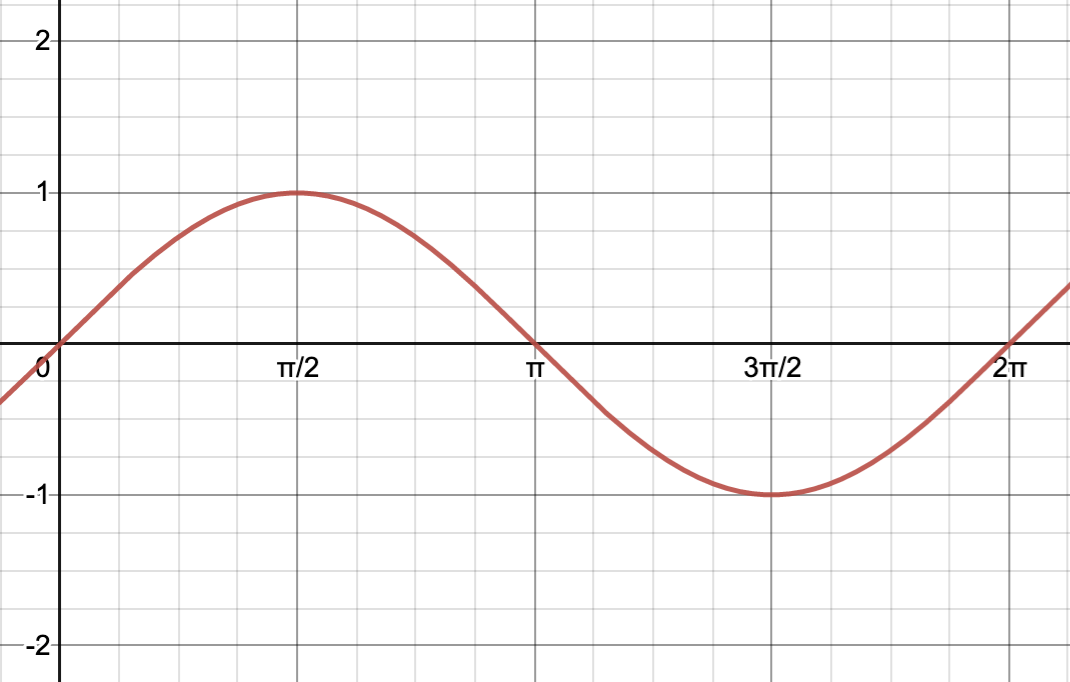
\includegraphics[width=\textwidth]{figures/sine-wave-form.png}
	\caption{A basic sine wave}
	\label{fig:basic-sine-wave}
\end{figure}


\subsection{Sine Waves}
The first of the basic period waves is the sine wave. The sine wave is a signal with only one frequency, and is based on the trigonometric sine function. On the unit circle, the trigonometric sine function of a phase angle $\theta$ is defined as the ratio of the length of the opposite side and the hypotenuse of a right triangle. [DIAGRAM OF UNIT CIRCLE] The unit circle, with a radius of 1, results in the sine function $sin\theta$ being equal to the y-value in Cartesian coordinates, where the hypotenuse of the right triangle that is formed meets the circle. [SHOW DIAGRAM OF THIS] A trigonometric sine wave can then be used to synthesize a sine wave audio signal. So, instead of calculating the sine function for a single value $x$, to create the sine wave signal the sine function is performed on a time vector $t = \{t_1, t_2, \dots, t_n\}$, with units in seconds. $sin(t) = \{sin(t_1), sin(t_2), \dots, sin(t_n)\}$. This gives us what we see in figure \ref	{fig:unit-circle}. The table below summarizes these transformations.

\begin{figure}
	\centering
	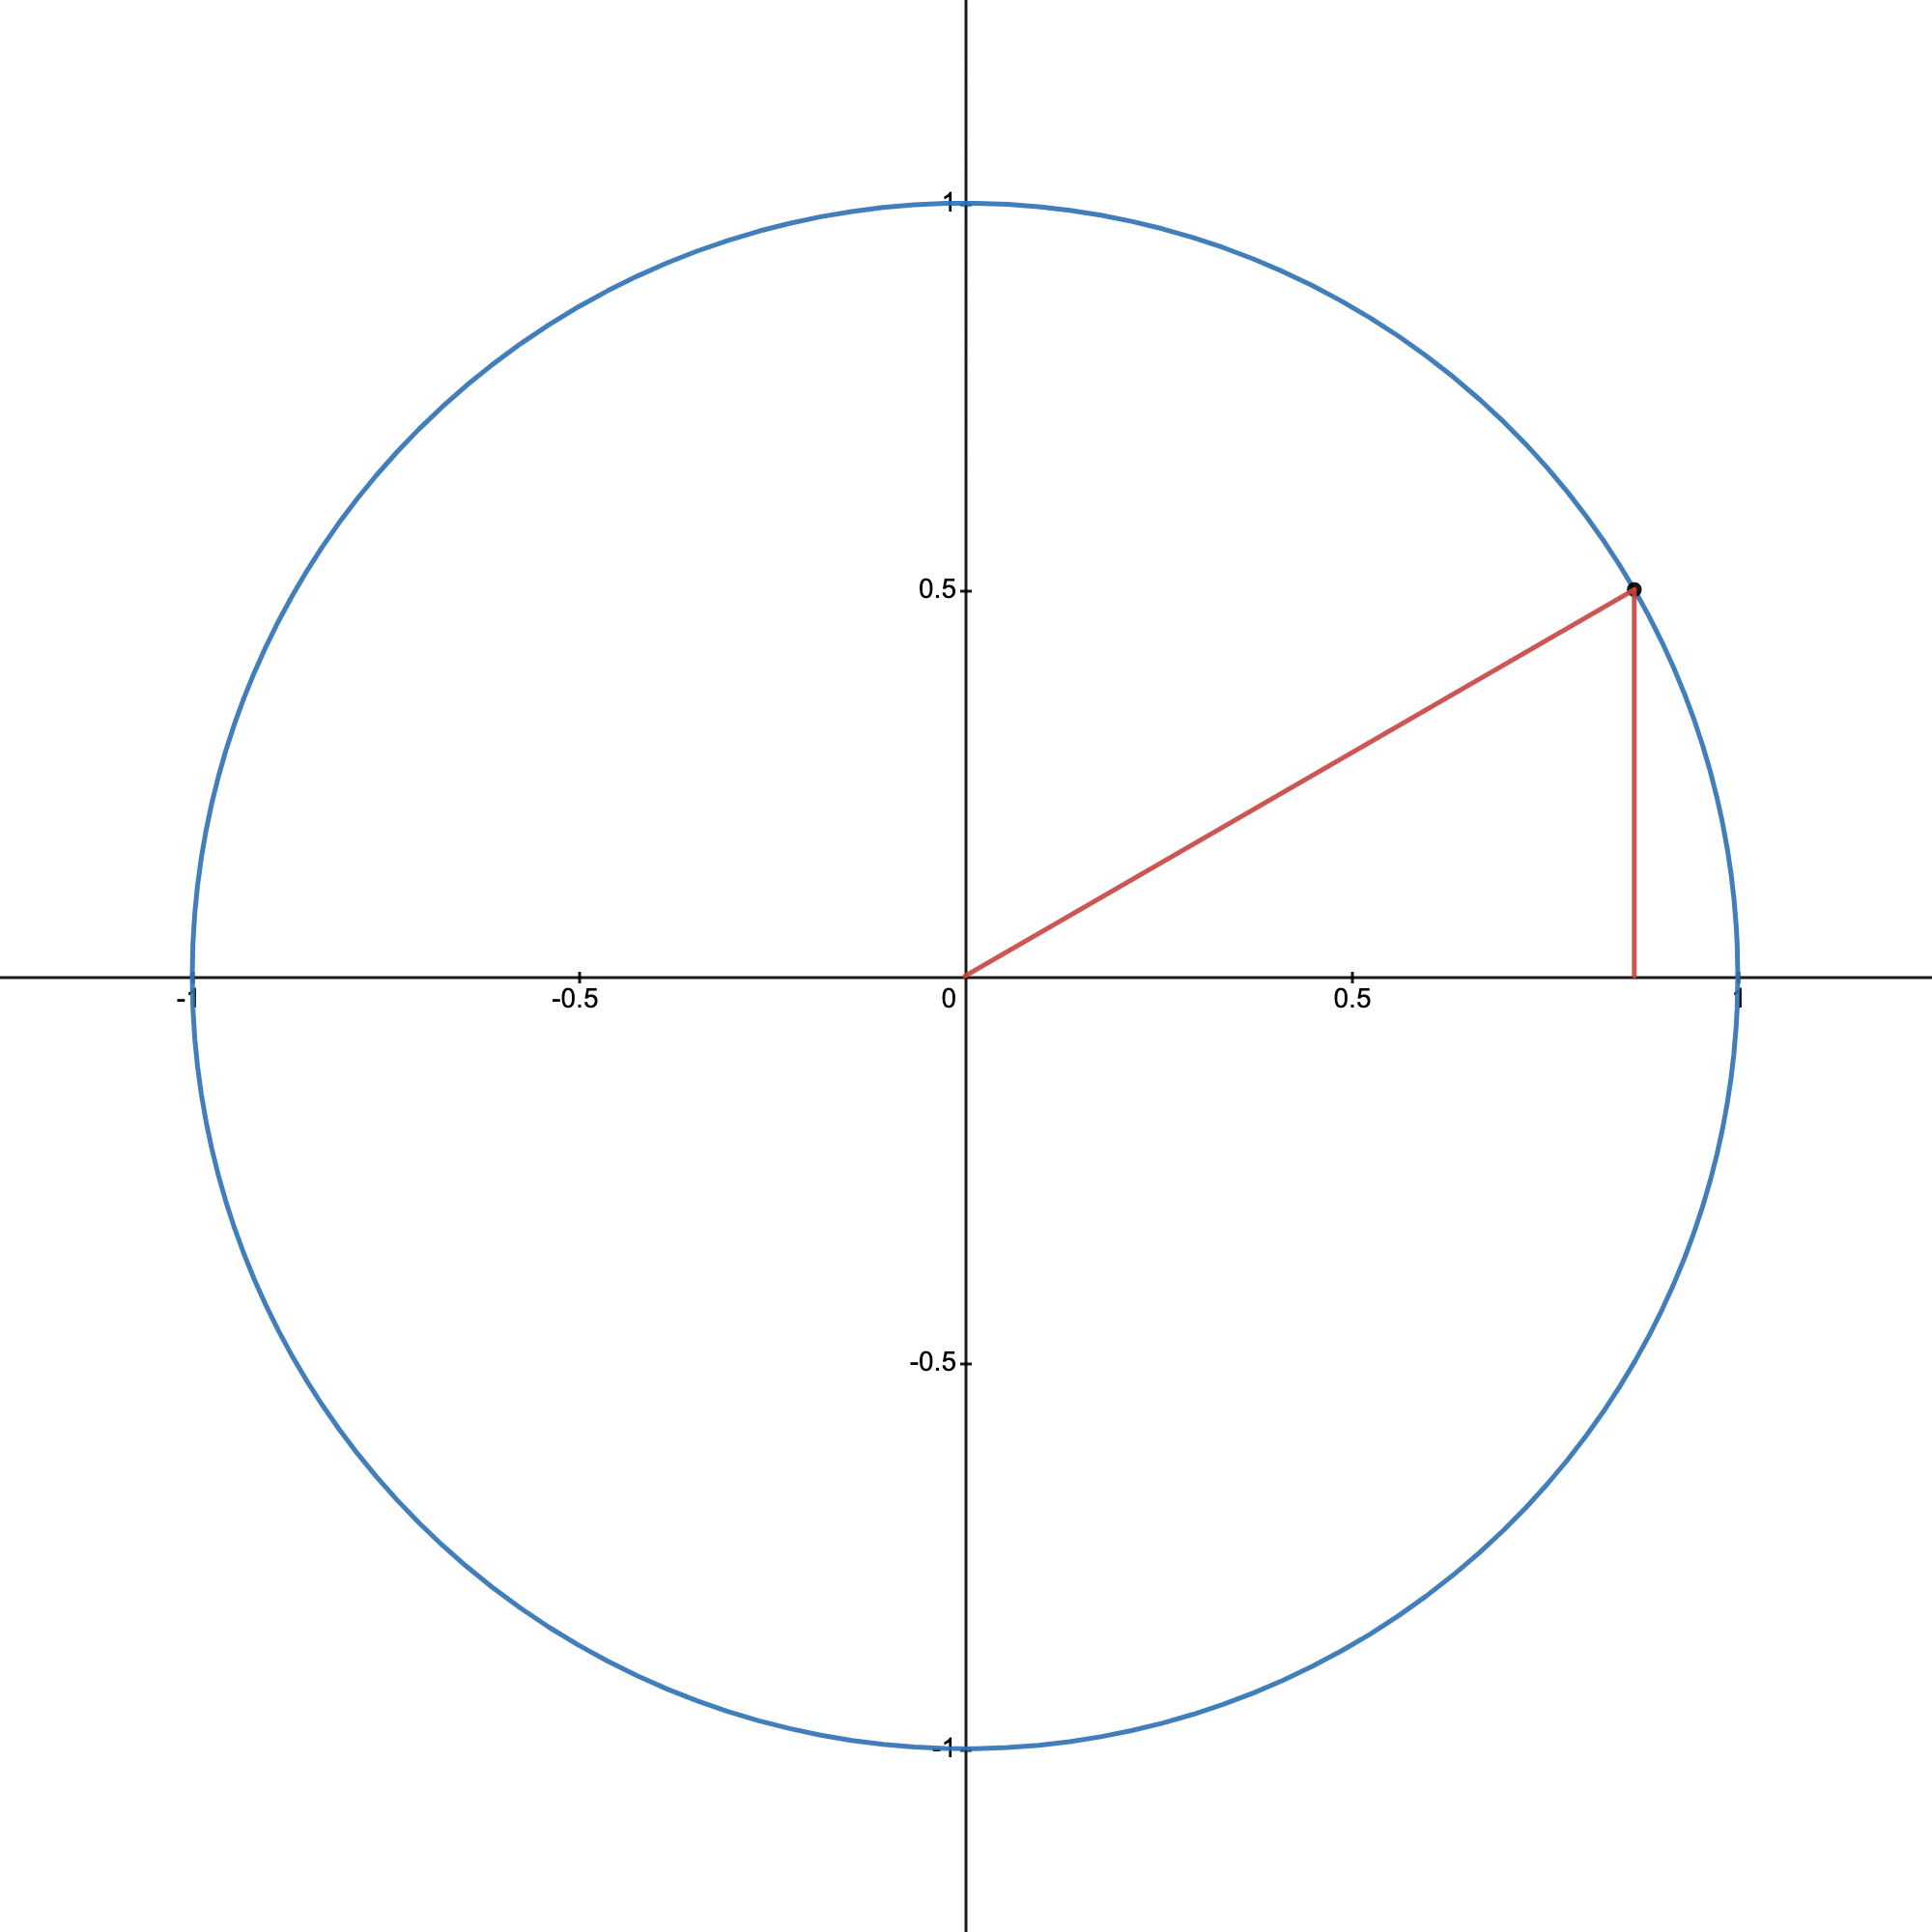
\includegraphics[width=0.5\textwidth]{figures/unit-circle.png}
	\caption{The unit circle}
	\label{fig:unit-circle}
\end{figure}

\begin{center}
    \begin{tabular}{c c}
        Function Input & Output Characteristics \\
        $sin(t)$ & $\frac{1 \textrm{ cycle}}{2\pi \textrm{ seconds}}$\\
        $sin(2\pi \cdot t)$ & $\frac{1 \textrm{ cycle}}{1 \textrm{ second}}$\\
        $sin(2\pi \cdot f \cdot t)$ & $\frac{f \textrm{ cycles}}{1 \textrm{ second}}$\\
        $sin(2\pi \cdot f \cdot t + \varphi)$ & Phase offset, $\varphi \varepsilon$ $[0, 2\pi]$\\
        $A \cdot sin(2\pi \cdot f \cdot t + \varphi)$ & Amplitude, \textit{A}
    \end{tabular}
\end{center}
The resulting sine wave signal can then be written as $x[t] = A \cdot sin(2 \cdot \pi \cdot f \cdot t + \theta$. $f$ is the frequency scalar, $t$ is the time vector of samples, and $\theta$ is the phase offset, between $[0, 2\pi]$.

\subsection{Square Waves}
The second of the periodic waves, the square wave, is a signal which oscillates between a singular positive value, and a single negative value \cite{Tarr_2019}. [INSERT DIAGRAM OF SQUARE WAVE]. An approximation of a square wave can be creating by combining multiple individual harmonics, or sine functions. This method of forming an audio signal is known as \textit{additive synthesis}, in which a new timbre is created by adding together sine waves. As a square wave is the summation of the odd-numbered harmonics, the following equation can be used \cite{Tarr_2019}.

\begin{align}
    \textrm{Let } x &= 2 \cdot \pi \cdot f \cdot t \\
    M &= \bigg \lfloor \frac{F_s}{2 \cdot f} \bigg \rfloor \\
    \textrm{square}(x) &= \frac{4}{\pi}(sin(x) + \frac{1}{3}sin(3 \cdot x) + \frac{1}{5}sin(5 \cdot x) + \dots) \\
    \textrm{square}(x) &= \frac{4}{\pi}\sum_{n=1, 3, 5, \dots}^{M}(n \cdot x)
\end{align}

Thus, the value \textit{M} is the harmonic with the highest frequency. This is calculated to be the number of odd harmonics less than the Nyquist frequency of $\frac{F_S}{2}$, rounded down to the nearest whole number. [INSERT DEF OF NYQUIST FREQ]

\subsection{Sawtooth Waves}
A Sawtooth wave is a signal with an amplitude which changes linearly between a minimum value, and a maximum value. [DIAGRAM SAWTOOTH HERE] Sawtooth waves are also created through additive synthesis, combining multiple sine functions together to create it. We have a similar equation to the one for square waves. 

\begin{align}
    \textrm{Let } x &= 2 \cdot \pi \cdot f \cdot t \\
    M &= \bigg \lfloor \frac{F_s}{2 \cdot f} \bigg \rfloor \\
    \textrm{square}(x) &= \frac{1}{2} - \frac{1}{\pi}(sin(x) + \frac{1}{2}sin(2 \cdot x) + \frac{1}{3}sin(3 \cdot x) + \dots) \\
    \textrm{square}(x) &= \frac{1}{2} - \frac{1}{\pi}\sum_{n=1}^{M}(\frac{1}{n}sin(n \cdot x)
\end{align}

One thing to notice, is the equations for saw tooth waves and square waves are very similar, with both waves being the summation of the odd harmonics of the fundamental frequency \cite{Tarr_2019}.

\section{Time Domain and Frequency Domain}

Digital signals are studied in one of four domains: time domain, spatial domain, frequency domain, and wavelet domain. For the purposes of this research, we focus most on only two of these domains: the time domain and the frequency domain. These domains are most commonly used in audio analysis and synthesis. Digital audio is normally viewed in the time domain, and through the use of the Discrete Fourier Transform (sometimes also called the Fast Fourier Transform), we are able to produce a frequency domain representation for frequency analysis.

\subsection{Time Domain}

Audio is most commonly represented as a waveform, most commonly as the sine wave, with time plotted against the wave's amplitude. The x-axis will represent the discrete audio signal, and is normalized to represent the hours, minutes, or seconds. Normalization is the process of transposing a data set to a specific reference value, by dividing the output value by a given constant \cite{Zjalic_2021}. In audio, the most common type of normalization will be applied to a common audio waveform, to produce a signal that is normalized between the values of 1 and -1. 1 thus becomes the reference value for positive values, and -1 for negative values. To normalize audio, the following formula is applied to an audio signal: sample value $\times$ $\frac{1}{\textrm{reference value }}$. Audio normalization is useful for audio analysis, in that it allows for comparisons to be made between signals, regardless of their magnitude and sample rate \footnote{[INSERT DEF OF SAMPLE RATES]}. The y-axis then represents the magnitude of each audio sample, in which the decibels (or another magnitude unit) are a bipolar normalized value, between a positive and negative value. 

To transform the time representation from samples to seconds, the sample rate must first be known. From there, it is simple to transpose \cite{Zjalic_2021}. For example, we assume that for the 44100 samples we have that the sample rate is also 44100 Hz [INSERT DEF OF HZ IF NOT IN ALREADY]. So, $44100 / 441100 = 1$ second, in that we divide the number of samples by the sample rate, to obtain a time representation in seconds. Another example may showcase this better. Assume we have 2646000 samples, and a sample rate of 44100 Hz. Then, we have $2646000/44100 = 60$ seconds.

\subsection{Frequency Domain}
The physical concept of frequency is relatively simple: it is the number of occurrences per unit of time in a given phenomenon \cite{Gabrielli_2020}. In audio, this becomes the number of repetitions, or cycles, of a sine wave. This type of frequency is known as the \textit{temporal frequency}, and will be denoted with the letter \textit{f}. For acoustic audio signals, we will be describing frequency in Hertz (H).\footnote{The reciprocal of the temporal frequency is known as the period, denoted as capital \textit{T}. This is defined as the time required to completed one full cycle at any given frequency, otherwise known as $T = \frac{1}{\textit{f}}$.} In digital signal processing, we instead will be using angular frequency (radians per second, denoted with $\omega$), which measures the angular displacement per unit of time. Thus, we have the following relation between temporal frequency, angular frequency, and period \cite{Gabrielli_2020}.

\begin{align}
    f &= \frac{\omega}{2\pi} &w &= 2\pi &f &= \frac{2\pi}{T}
\end{align}

To convert a signal into the frequency domain, and to obtain its frequency components, the Fourier Transform can be used\footnote{The Inverse Fourier Transform can be used to go from the frequency domain to the time domain.}. Transforms like these are common in audio signal processing. These are mathematical operations which allow you to observe a signal from a different perspective\footnote{The result of a transform on an audio signal can be seen in figure 2.9 of Gabrielli.}.

\section{The Fourier Transform}
Joseph Fourier (1768-1830) stated that all sounds could be represented by one or more sine waves of various frequencies, amplitudes, durations, and phases. Any sound could then be broken down into its component parts, and analyzed with Fourier analysis \cite{Winer_2018}. 

The Fourier transform converts the time information to a magnitude and phase component of each frequency. With the Fourier transform, Fourier stated that any signal \textit{x} of time length \textit{t} can be broken down into the sine and cosine waves of which it is composed \cite{Zjalic_2021}, each having \textit{t} cycles. Thus, based on the properties of the specific audio signal, the Fourier Transform can be broken into four methods:

\begin{enumerate}
    \item Fourier Transform: applies to continuous signals which are aperiodic (without periodic repetitions)
    \item Fourier Series: applies to continuous, periodic signals
    \item Discrete Time Fourier Transform: applies to discrete signals\footnote{A signal which is defined at discrete points between positive and negative values} which are also aperiodic
    \item Discrete Fourier Transform: applies to discrete signals which are also periodic
\end{enumerate}

Digital data, and so digital audio, has no relation to the first two methods. Sine and cosine waves in audio are defined from negative to positive infinity. So, by imagining a sine or cosine wave as simply one repetition of a series of a periodic sinusoidal, the criteria for a Discrete Fourier Transform is met \cite{Zjalic_2021}. Thus, it is the only transform that is applicable to digital audio signal processing, as it is both discrete and periodic.

\subsection{Discrete Fourier Transform}
The Discrete Fourier Transform (or DFT) takes the audio samples in the time domain as an input, and outputs two frequency domain outputs: $\frac{N}{2} + 1$ points. These outputs represent the amplitude of the sine and cosine waves, with \textit{N} the number of samples in the input, giving us the equation below \cite{Gold_Morgan_Ellis_2011}. This equation is of a finite duration sequence x(n)
with $0 \leq n \leq N + 1$.

\begin{equation}\label{eq:dft-equation}
    X[k] = \sum_{k=0}^{N+1}x[n]e^{-j (\frac{2\pi}{N})kn}
\end{equation}

The Discrete Fourier Transform represents the vector $x[n]$ as a combination of harmonically-related sinusoidals. 

\section{Audio Manipulations}